\begin{frame}{The Ship of Theseus}
  \setlength{\intextsep}{0.5em}

  \only<1>{
    \begin{figure}
      \centering
      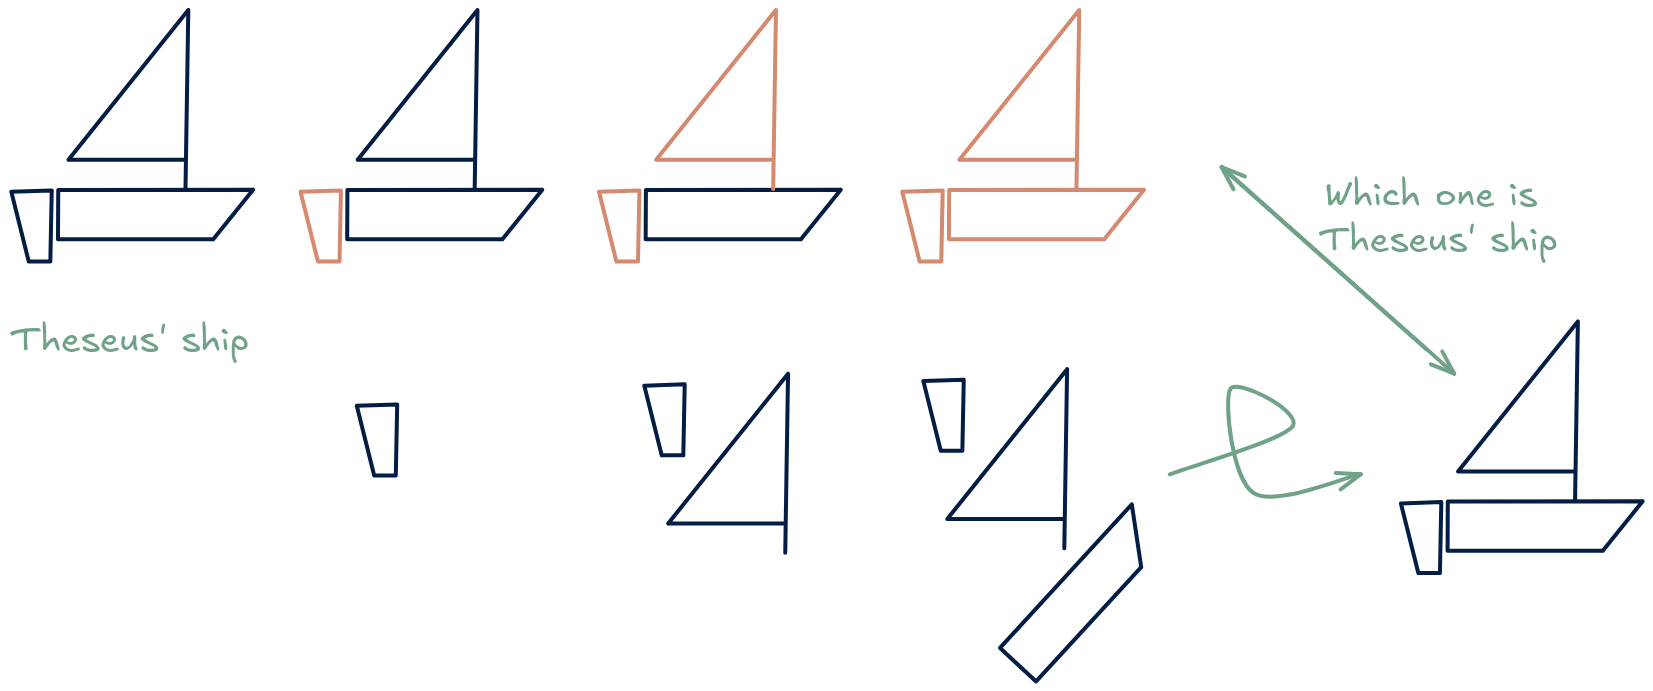
\includegraphics[width=0.85\textwidth, height=0.65\textheight, keepaspectratio]{slides/theseus/paradox/figs/ship-of-theseus-1.png}
      \caption{Planks replaced one by one, spare parts assembled into a second ship.}
    \end{figure}
  }

  \only<2>{
    \begin{figure}
      \centering
      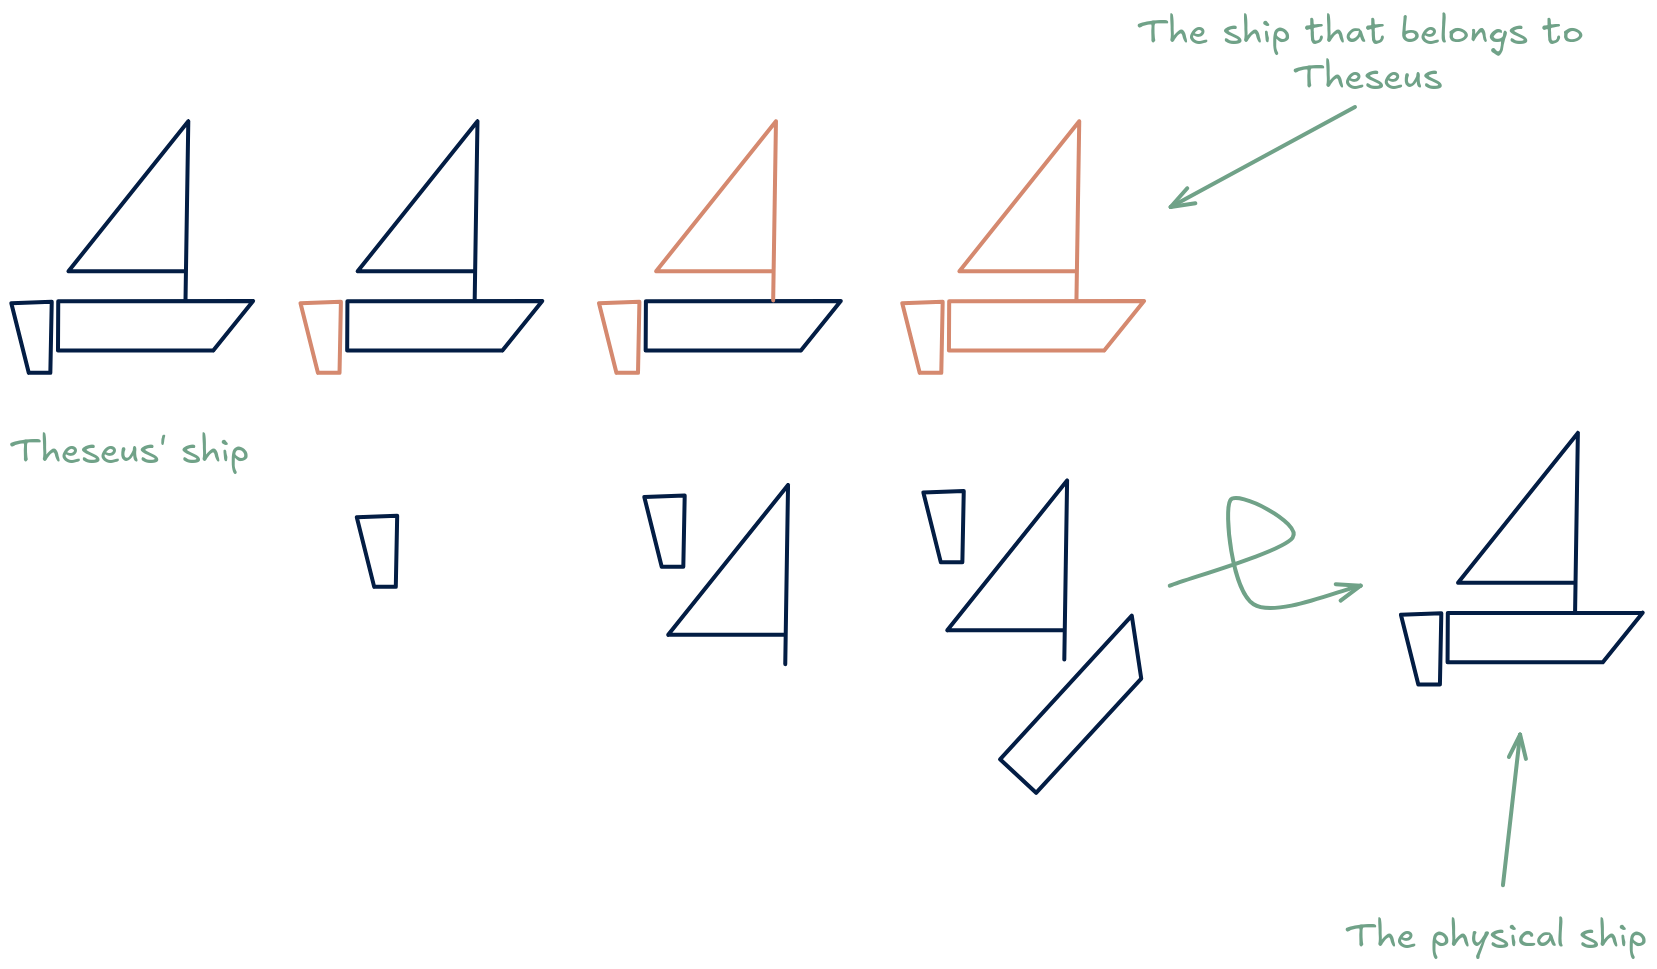
\includegraphics[width=0.85\textwidth, height=0.65\textheight, keepaspectratio]{slides/theseus/paradox/figs/ship-of-theseus-2.png}
      \caption{Two perspectives: the ship that \emph{belongs} to Theseus, and the \emph{physical} ship made of the original planks.}
    \end{figure}
  }

  \only<3>{
    \begin{figure}
      \centering
      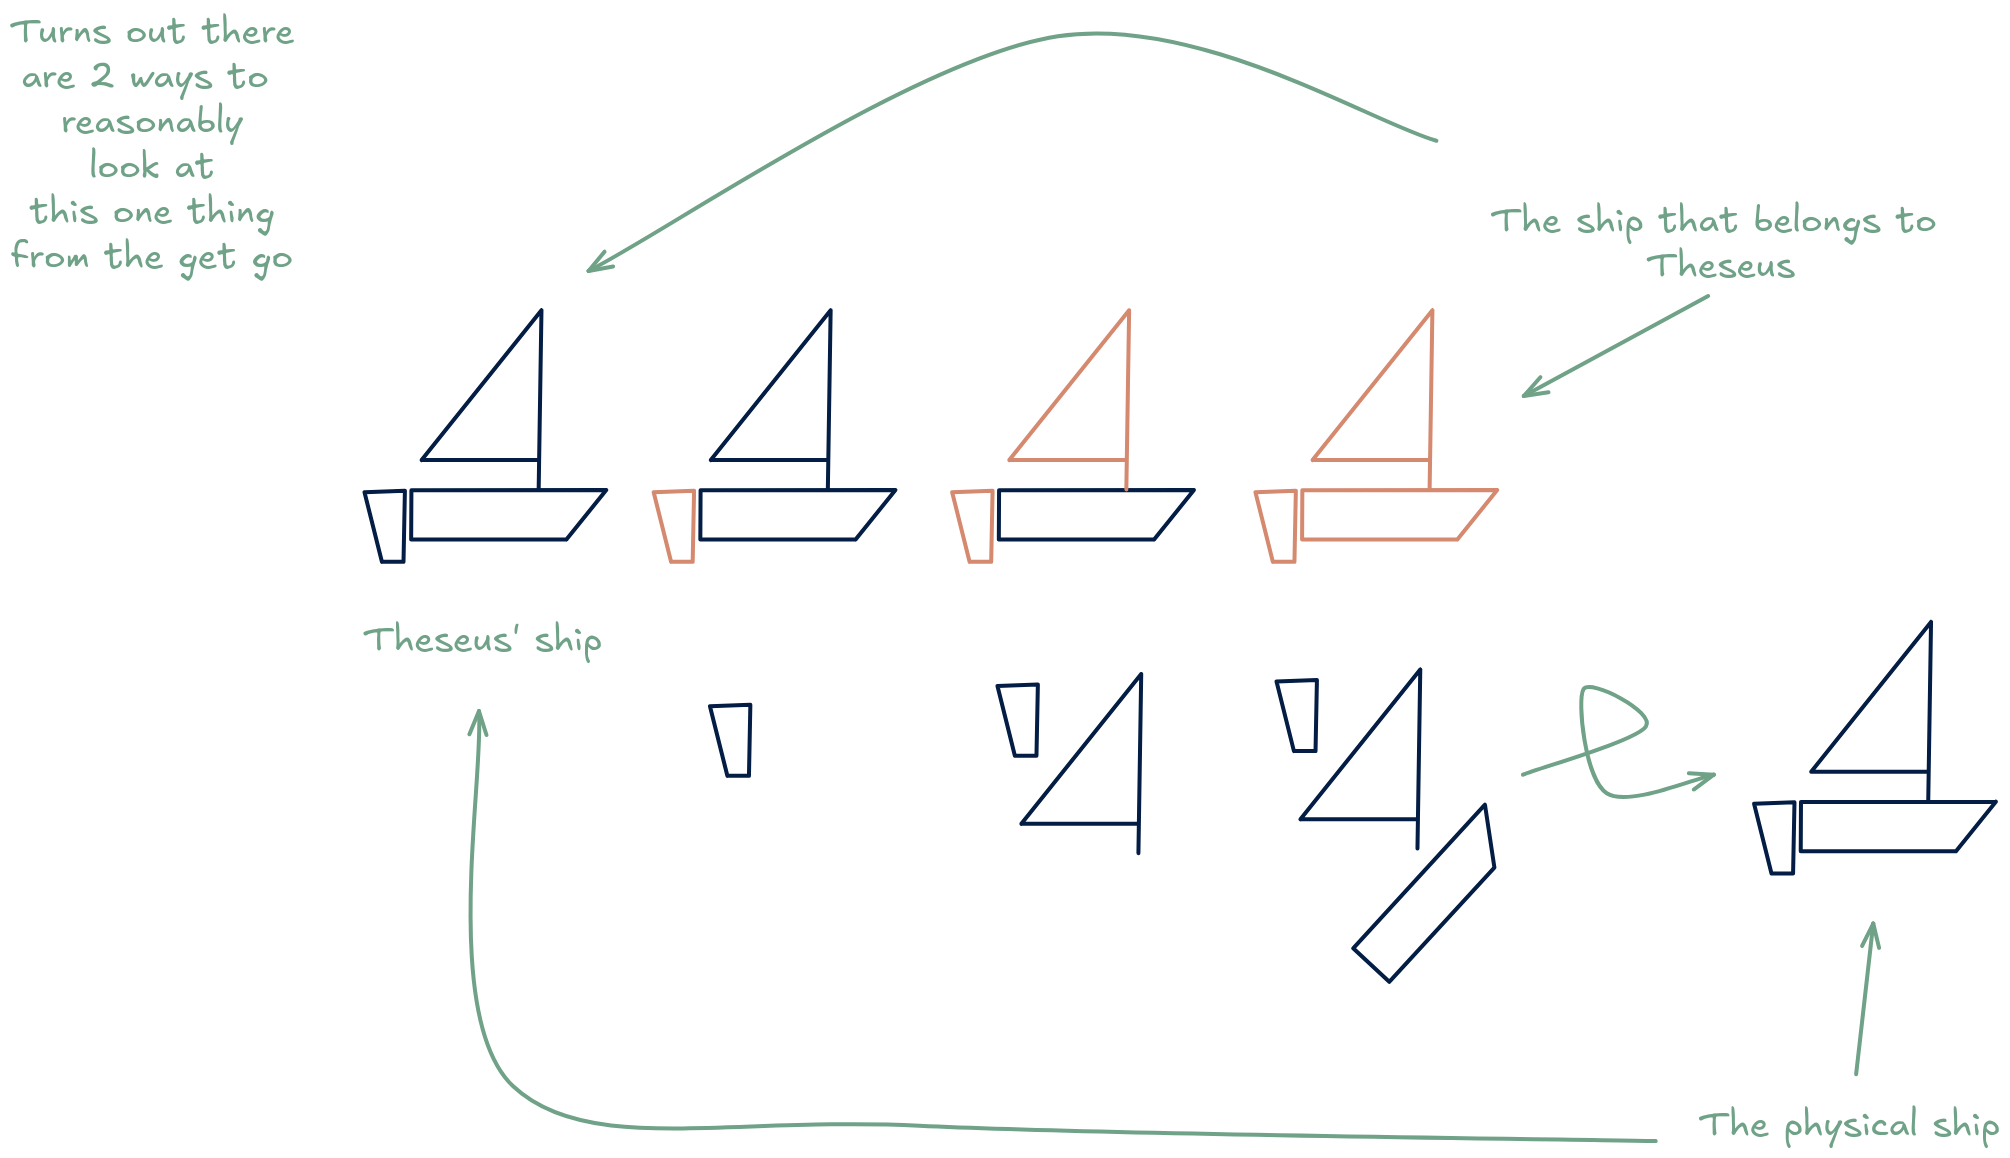
\includegraphics[width=0.85\textwidth, height=0.65\textheight, keepaspectratio]{slides/theseus/paradox/figs/ship-of-theseus-3.png}
      \caption{Turns out there are two (or more) ways to reasonably look at this one thing — from the get-go.}
    \end{figure}
  }
\end{frame}

\begin{frame}{Market services add an extra layer of interpretation}
  \setlength{\intextsep}{0.5em}

  \begin{figure}
    \centering
    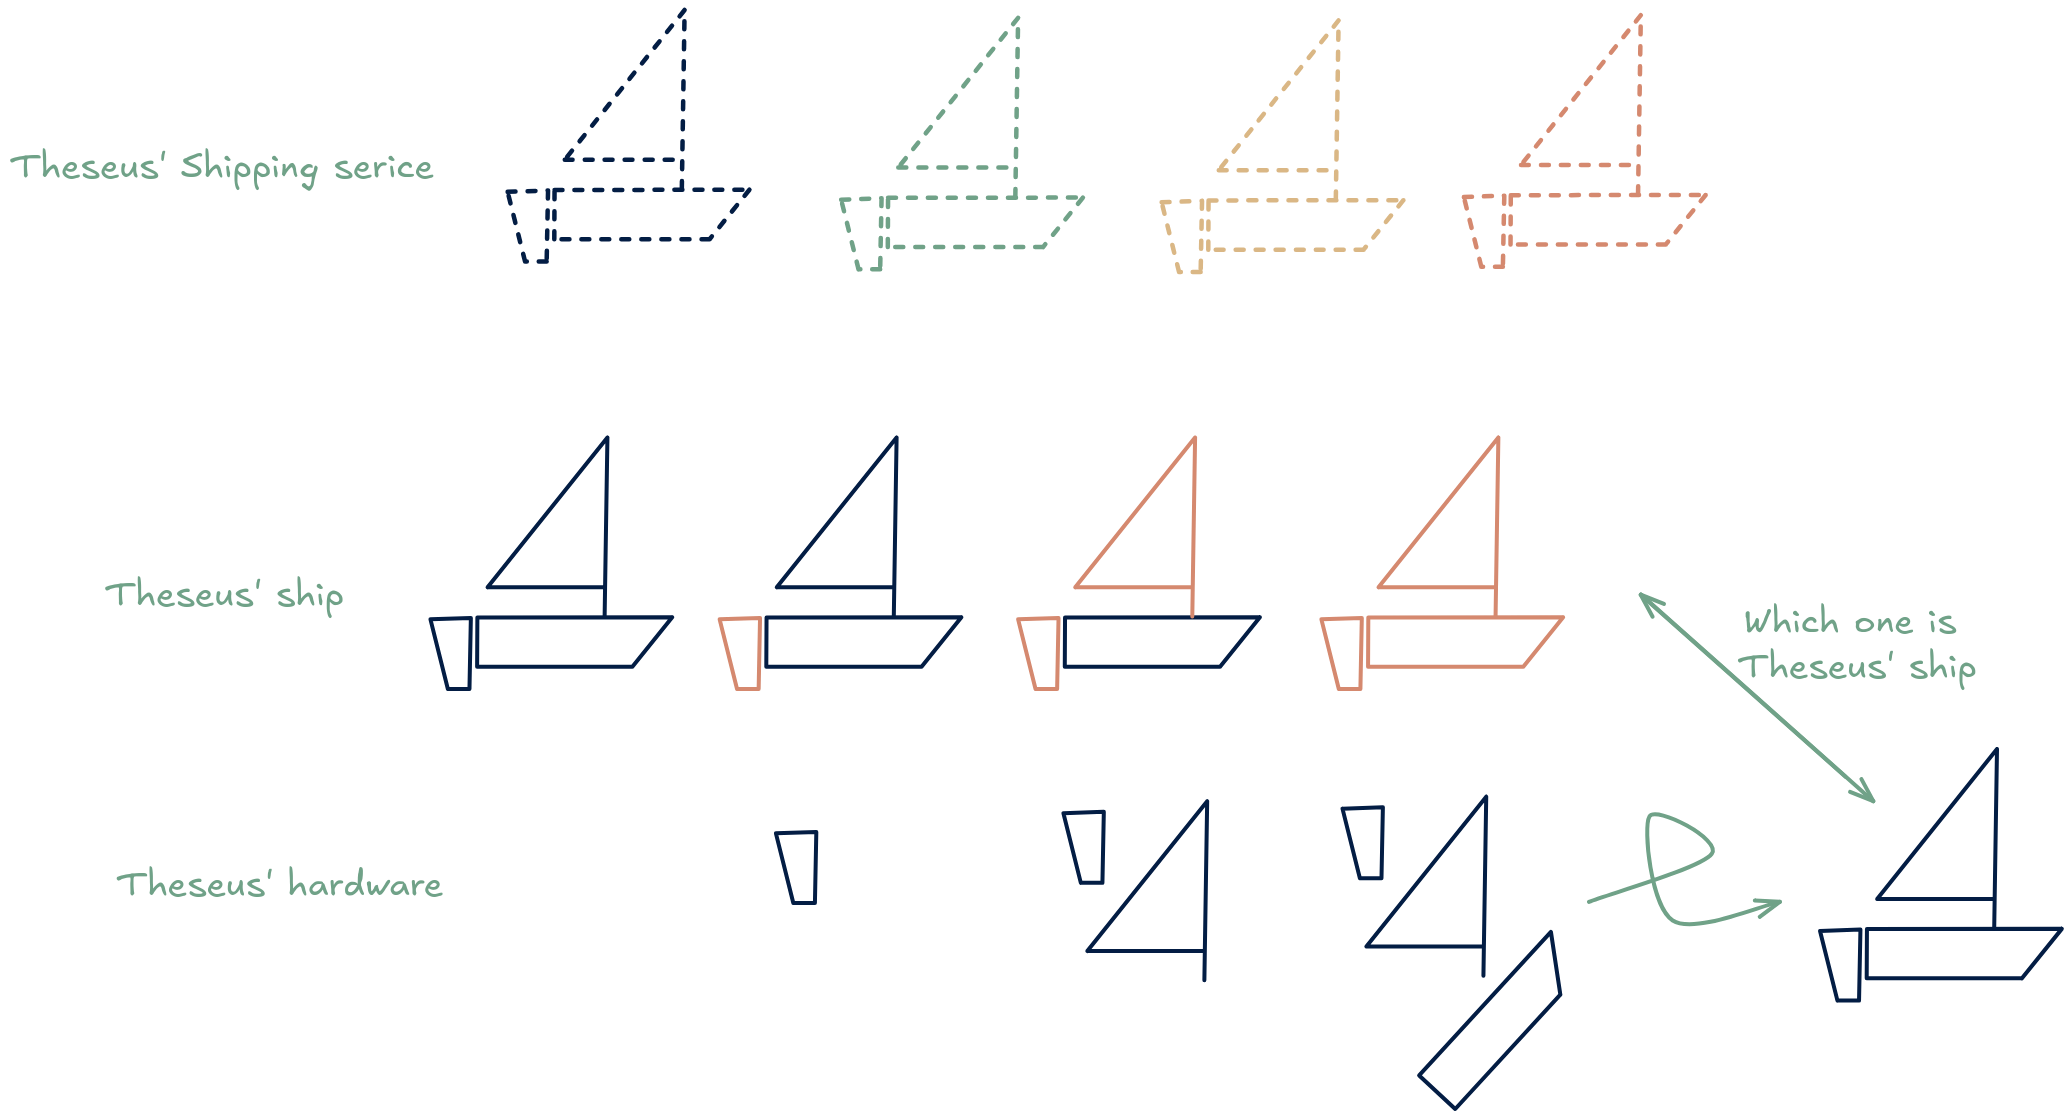
\includegraphics[width=0.85\textwidth, height=0.65\textheight, keepaspectratio]{slides/theseus/paradox/figs/shipping-service-of-theseus.png}
    \caption{Three levels of the ship of \emph{Theseus}: the shipping service, the ship, and the hardware — and still the question ``which one is Theseus' ship?''}
  \end{figure}
\end{frame}
